%---- Required Packages and Functions ----

\documentclass[a4paper,11pt]{article}
\usepackage{latexsym}
\usepackage{xcolor}
\usepackage{float}
\usepackage{ragged2e}
\usepackage[empty]{fullpage}
\usepackage{wrapfig}
\usepackage{lipsum}
\usepackage{tabularx}
\usepackage{titlesec}
\usepackage{geometry}
\usepackage{marvosym}
\usepackage{verbatim}
\usepackage{enumitem}
\usepackage{fancyhdr}
\usepackage{multicol}
\usepackage{graphicx}
\usepackage{cfr-lm}
\usepackage[T1]{fontenc}
\usepackage[colorlinks=true, linkcolor=blue, urlcolor=blue]{hyperref} % << Only keep this one

\setlength{\footskip}{10pt}  % fix fancyhdr warning
\setlength{\multicolsep}{0pt} 
\pagestyle{fancy}
\fancyhf{} % clear all header and footer fields
\fancyfoot{}
\renewcommand{\headrulewidth}{0pt}
\renewcommand{\footrulewidth}{0pt}
\geometry{left=1.4cm, top=0.8cm, right=1.2cm, bottom=1cm}


\usepackage[most]{tcolorbox}

\tcbset{
	frame code={},
	center title,
	left=0pt,
	right=0pt,
	top=0pt,
	bottom=0pt,
	colback=gray!20,
	colframe=white,
	width=\dimexpr\textwidth\relax,
	enlarge left by=-2mm,
	boxsep=4pt,
	arc=0pt,outer arc=0pt,
}

\urlstyle{same}
\raggedright
\setlength{\tabcolsep}{0in}

% Sections formatting
\titleformat{\section}{
  \vspace{-4pt}\scshape\raggedright\large
}{}{0em}{}[\color{black}\titlerule \vspace{-7pt}]

%-------------------------
% Custom commands
\newcommand{\resumeItem}[2]{
  \item{
    \textbf{#1}{:\hspace{0.5mm}#2 \vspace{-0.5mm}}
  }
}

\newcommand{\resumePOR}[3]{
\vspace{0.5mm}\item
    \begin{tabular*}{0.97\textwidth}[t]{l@{\extracolsep{\fill}}r}
        \textbf{#1},\hspace{0.3mm}#2 & \textit{\small{#3}} 
    \end{tabular*}
    \vspace{-2mm}
}

\newcommand{\resumeSubheading}[4]{
\vspace{0.5mm}\item
    \begin{tabular*}{0.98\textwidth}[t]{l@{\extracolsep{\fill}}r}
        \textbf{#1} & \textit{\footnotesize{#4}} \\
        \textit{\footnotesize{#3}} &  \footnotesize{#2}\\
    \end{tabular*}
    \vspace{-2.4mm}
}

\newcommand{\resumeProject}[4]{
\vspace{0.5mm}\item
    \begin{tabular*}{0.98\textwidth}[t]{l@{\extracolsep{\fill}}r}
        \textbf{#1} & \textit{\footnotesize{#3}} \\
        \footnotesize{\textit{#2}} & \footnotesize{#4}
    \end{tabular*}
    \vspace{-2.4mm}
}

\newcommand{\resumeSubItem}[2]{\resumeItem{#1}{#2}\vspace{-4pt}}

% \renewcommand{\labelitemii}{$\circ$}
\renewcommand{\labelitemi}{$\vcenter{\hbox{\tiny$\bullet$}}$}

\newcommand{\resumeSubHeadingListStart}{\begin{itemize}[leftmargin=*,labelsep=0mm]}
\newcommand{\resumeHeadingSkillStart}{\begin{itemize}[leftmargin=*,itemsep=1.7mm, rightmargin=2ex]}
\newcommand{\resumeItemListStart}{\begin{justify}\begin{itemize}[leftmargin=3ex, rightmargin=2ex, noitemsep,labelsep=1.2mm,itemsep=0mm]\small}

\newcommand{\resumeSubHeadingListEnd}{\end{itemize}\vspace{2mm}}
\newcommand{\resumeHeadingSkillEnd}{\end{itemize}\vspace{-2mm}}
\newcommand{\resumeItemListEnd}{\end{itemize}\end{justify}\vspace{-2mm}}
\newcommand{\cvsection}[1]{%
\vspace{2mm}
\begin{tcolorbox}
    \textbf{\large #1}
\end{tcolorbox}
    \vspace{-4mm}
}

\newcolumntype{L}{>{\raggedright\arraybackslash}X}%
\newcolumntype{R}{>{\raggedleft\arraybackslash}X}%
\newcolumntype{C}{>{\centering\arraybackslash}X}%
%---- End of Packages and Functions ------

%-------------------------------------------
%%%%%%  CV STARTS HERE  %%%%%%%%%%%
%%%%%% DEFINE ELEMENTS HERE %%%%%%%
\newcommand{\name}{Vaibhav Arora} % Your Name
\newcommand{\course}{B.Tech - Computer Science and Engineering} % Your Course
\newcommand{\roll}{12041650} % Your Roll No.
\newcommand{\phone}{8168401709} % Your Phone Number
\newcommand{\phonee}{920653140} % Your Phone Number
\newcommand{\emaila}{vaibhav.arora@tecnico.ulisboa.pt} %Email 1
\newcommand{\emailb}{vaibhavarora2182@gmail.com} %Email 2
\newcommand{\github}{Vaibhav-Arora-2182} %Github
\newcommand{\website}{https://github.com/Vaibhav-Arora-2182} %Website
\newcommand{\linkedin}{Vaibhav Arora} %linkedin




\begin{document}
\fontfamily{cmr}\selectfont
%----------HEADING-----------------
\begin{tabular}{@{} l l @{}}
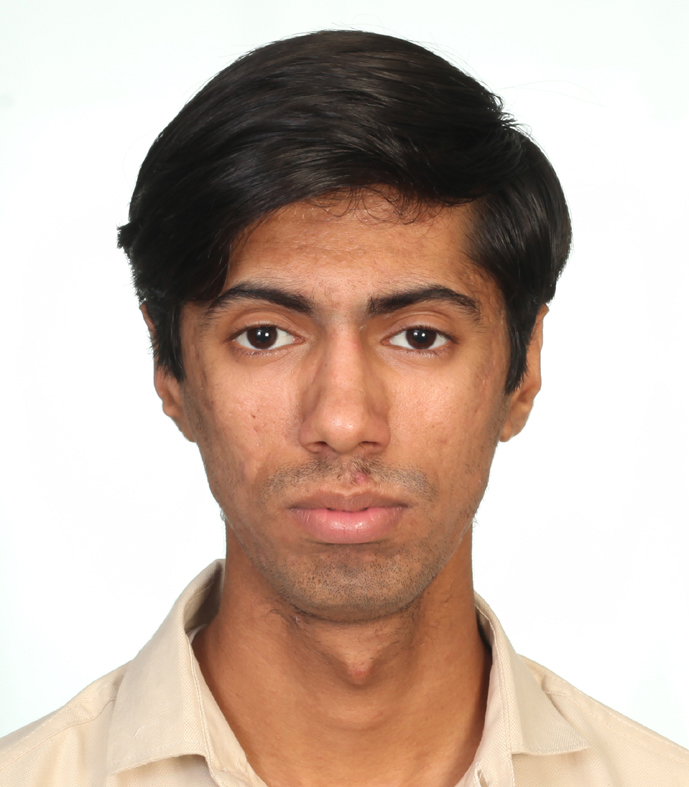
\includegraphics[width=2.3cm,clip]{22.jpg} & \\[0.3em]

\textbf{\LARGE \name} & \\[0.3em]

\textbf{PhD Candidate:} & Distributed Systems and Fault Tolerance (\textbf{DPSS, INESC-ID}) \\
& Instituto Superior Técnico, Universidade de Lisboa \\
\textbf{Research Focus:} & Development of \textbf{ByzPlug}, an implementation-agnostic fault injection framework \\
& to assess safety, liveness, and performance of \\
& Byzantine Fault Tolerant blockchain consensus under adverse conditions. \\



\textbf{Phone (IN):} & +91-\phone \\

\textbf{Phone (PT):} & +351-\phonee \\

\textbf{Email 1:} & \href{mailto:\emaila}{\emaila} \\

\textbf{Email 2:} & \href{mailto:\emailb}{\emailb} \\[0.3em]

\textbf{Github:} & \href{https://github.com/Vaibhav-Arora-2182\github}{github.com/Vaibhav-Arora-2182} \\

\textbf{LinkedIn:} & \href{https://www.linkedin.com/in/vaibhav-arora-a0929b18a/\linkedin/}{linkedin.com/in/\linkedin} \\
\end{tabular}



\section*{About Me}

I research distributed learning and Byzantine fault-tolerant consensus in blockchain networks. My federated learning work focuses on asynchronous, cluster-based aggregation resilient to non-IID data, partial participation, and adversarial poisoning, leveraging embedding-level KL divergence and decentralized knowledge distillation.

Currently, I develop \textbf{ByzPlug}, a programmable fault injection framework for BFT protocols like QBFT in Hyperledger Besu. ByzPlug enables stateful manipulation of DevP2P/RLPx traffic, simulating equivocation, replay, and view-change corruption to evaluate consensus safety and liveness under asynchronous, adversarial conditions.

My goal is to build scalable, verifiable infrastructure for secure decentralized computation spanning learning and consensus.

\vspace{0.5em}
\noindent\textbf{Supervisors:} 
\href{https://www.dpss.inesc-id.pt/~rodrigo/}{Prof. Rodrigo Rodrigues} \quad | \quad 
\href{https://miguelmatos.me}{Prof. Miguel Matos} \quad | \quad 
\href{https://sites.google.com/iitbhilai.ac.in/subhajit}{Prof. Subhajit Sidhanta (B. Tech.)}

\section{Experience}
\resumeSubHeadingListStart

\resumeSubheading
{INESC-ID, Instituto Superior Técnico – Universidade de Lisboa}{}
{Junior Researcher}{October, 2024 – Present}
\vspace{-0.5em}
\resumeItemListStart
  \item {Working on \textbf{Testing and Comparing Real-World Blockchains Under Strain} under Prof. Rodrigo Rodrigues and Prof. Miguel Matos}
  \item {Developed ByzPlug: an implementation-agnostic fault injection framework to evaluate BFT protocols (QBFT, HotStuff, Tendermint)}
  \item {Built packet-level introspection tools to analyze liveness, safety, and performance under adversarial network conditions}
\resumeItemListEnd

\resumeSubheading
{Indian Institute of Technology, Bhilai}{}
{Teacher’s Assistant – CS102 (Data Structures)}{February, 2023 – April, 2023}
\vspace{-0.5em}
\resumeItemListStart
  \item {Assisted Dr. Amit Kumar Dhar in teaching the Data Structures course at IIT Bhilai}
  \item {Prepared model solutions for assignments and examinations, and evaluated student submissions}
  \item {Provided individual feedback and mentoring to enrolled students}
\resumeItemListEnd

\resumeSubheading
{Technology Innovation Hub, IIT Bhilai}{}
{Research Fellow – Graph Learning on Bitcoin Dataset}{February, 2022 – July, 2022}
\vspace{-0.5em}
\resumeItemListStart
  \item {Performed exploratory data analysis on the Elliptic Bitcoin dataset using \texttt{networkx} and \texttt{Neo4j}}
  \item {Studied and implemented temporal graph learning frameworks including EvolveGCN}
  \item {Investigated anomaly detection techniques for crypto transaction networks}
\resumeItemListEnd

\resumeSubHeadingListEnd
\vspace{-5.5mm}



% \section{About Me}
% Having explored various domains such as Distributed Systems, Machine Learning, Cryptography etc. in my Bachelors, I am ideally suited for a multi-faceted perspective on whatever projects I undertake. My recent work lies in the development of Fault Tolerant algorithms for Asynchronous Federated Learning which piqued my interest in the domain of Distributed Systems. And hence, I plan to work on Byzantine Fault Tolerance as I want to contribute in improving the robustness of the underlying consensus algorithms, which is the backbone of present Block-chain systems. 
%\rule{\textwidth}{0.1em}


\section*{Education}

\textbf{Doctorate Researcher}, INESC-ID, Instituto Superior Técnico, University of Lisbon \\
\textit{Ph.D. in Computer Science} \hfill Oct 2024 -- Present \\
Status: Ongoing

\vspace{4pt}

\textbf{Bachelor of Technology (Honors)}, Indian Institute of Technology, Bhilai \\
\textit{Major: Computer Science and Engineering} \hfill Graduated: 2024 \\
CGPA: 8.64 / 10.00

\vspace{4pt}

\textbf{Senior Secondary}, Central Board of Secondary Education (CBSE) \\
\textit{Stream: Science with Mathematics} \hfill Graduated: 2020 \\
Score: 97%

\vspace{4pt}

\textbf{Secondary School}, Central Board of Secondary Education (CBSE) \\
\hfill Graduated: 2018 \\
Score: 91%

\vspace{-2mm}

\section{Technical Skills}
\resumeHeadingSkillStart

\resumeSubItem{Programming Languages} 
  {Python, C/C++, Java, Bash, SQL, CUDA, Solidity}

\resumeSubItem{Distributed Systems \& RPC} 
  {gRPC, Hadoop, Spark, Hive Kafka, , NS-3 network simulation}

\resumeSubItem{Blockchain \& Consensus Protocols} 
  {Ethereum (DevP2P, RLPx, EVM), Hyperledger Besu (QBFT), Smart Contracts (Solidity), ByzPlug fault injection framework, cryptographic primitives (ECDSA, ECIES)}

\resumeSubItem{Machine Learning \& Frameworks} 
  {TensorFlow, PyTorch, PyTorch Geometric, DGL, Flower FL, scikit-learn, Keras}

\resumeSubItem{Data Processing \& Analytics} 
  {NumPy, Pandas, NetworkX, Neo4j, InfluxDB, MySQL, Hadoop, Spark, Hive, BigQuery}

\resumeSubItem{Visualization \& Monitoring} 
  {Matplotlib, Seaborn, Plotly, Dash, TensorBoard, Weights \& Biases (WanDB)}

\resumeSubItem{Cryptography \& Security} 
  {PyCryptodome, OpenSSL, TLS, zero-knowledge proofs (basic)}

\resumeSubItem{DevOps \& Cloud} 
  {Docker, Kubernetes, Google Cloud Platform (GCP), AWS (EC2, DataProc, S3)}

\resumeSubItem{Miscellaneous} 
  {Git, Wireshark, LaTeX, OpenCV, NLTK, GurobiPy, Sagemath, Tkinter, Pillow}

\resumeHeadingSkillEnd

%-----------PROJECTS-----------------
\section{Personal projects}
\resumeSubHeadingListStart
\resumeSubheading
{Fault Tolerant Asynchronous Federated Learning}{}
{\phantom{under Dr. Subhajit Sidhanta}}{\phantom{February, 2023 - April, 2023}}
\vspace{-1.5 em}
\resumeItemListStart
\item {Laid out the functional requirements and premise of the problem statement by conducting extensive survey}
\item {Implemented Asynchronous Federated learning from scratch using Pytorch, gRPCs and multithreading}
\item {Devised a novel aggregation algorithm for handling client failures in Async FL and tested them against SOTA algorithms} 
\resumeItemListEnd
\resumeSubHeadingListEnd
\vspace{-5.5mm}


\resumeSubHeadingListStart
\resumeSubheading
{Optimization for Iterated Prisoners Dilemma}{}
{\phantom{under Dr. Subhajit Sidhanta}}{\phantom{February, 2023 - April, 2023}}
\vspace{-1.5 em}
\resumeItemListStart
\item {Simulated the multi agent iterated prisoner's dilemma and implemented various heuristic agents }
\item {Devised and implemented an effective fitness and action function for the GA-agents}
\item {Performed bench-marking of the implemented function against heuristic agents}
\resumeItemListEnd
\resumeSubHeadingListEnd
\vspace{-5.5mm}

\resumeSubHeadingListStart
\resumeSubheading
{Cobble detection at Bhilai Steel Plant}{}
{\phantom{under Dr. Subhajit Sidhanta}}{\phantom{February, 2023 - April, 2023}}
\vspace{-1.5 em}
\resumeItemListStart
\item {Performed Exploratory Data Analysis on the the multivariate Time Series data from IoT signals and video feed}
\item {Implemented MCUSUM, LSTM AutoEncoder and PCA for Time Series Anomaly detection}
\item {Implemented KLL Summarization algorithm to reduce the Volume on data and built a Telegraf dashboard to visualize the data from the InfluxDB database }
\resumeItemListEnd
\resumeSubHeadingListEnd
\vspace{-5.5mm}


%\section{Key courses taken}
%\resumeHeadingSkillStart
% \resumeSubItem{Computer Science} % Category
%    {Data Structures and Algorithms in Python, Discrete structures, Database Management Systems, Operating Systems, Introduction to Language Processing, Principles of Programming Languages, Introduction to Programing in Python, Computer Networks, Cryptography, Simulation of Biology, Computer Organization and Architecture}
%\resumeSubItem{Data Science and Artificial Intelligence}
% {Data Analytics and Vizualization, Machine Learning, Natural Language Processing, Management for Large Datasets (Audit), Statistical Programming (Audit)}
 
%\resumeSubItem{Miscellaneous}
%{Linear Algebra-1, Linear Algebra-2, Calculus-1, Calculus-2, Probability and Statistics, Quantum Physics, Electrodynamics, Introduction to Astronomy, Intrduction to Bioinformatics, Digital Farbrication}
%  \resumeSubItem{Electrical and Electronics} % Category
%     {Advanced Control Systems, Digital Systems, Microprocessors} % Skills
% \resumeHeadingSkillEnd

%-----------EXPERIENCE-----------------


%     \resumeSubheading
%       {Company A}{Bengaluru, India}
%       {API Developer \& Machine Learning Intern}{May. 2018 - Jul. 2018}
%       \resumeItemListStart
%     \item {XXXXXXXXXXXXXXX}
%         \item {YYYYYYYYYYYYYYYYYY}
%     \resumeItemListEnd

% \resumeSubHeadingListEnd
% \vspace{-5.5mm}
% \section{Key courses taken}
% \resumeHeadingSkillStart
% \resumeSubItem{Distributed Systems} % Category
% { : A}
% \resumeSubItem{Advanced Machine Learning} % Category
% { : A+}
% \resumeSubItem{Machine Learning} % Category
% { : A+}
% \resumeSubItem{Natural Language Processing} % Category
% { : A}
% \resumeSubItem{Data Structures} % Category
% { : A}

% \resumeSubItem{Data Analytics and visualization} % Category
% { : A}
% %\resumeSubItem{Computer Networks} % Category
% %{ : A-}
% %\resumeSubItem{Cryptography} % Category
% %{ : A-}
% \resumeHeadingSkillEnd
\section{Achievements}
\vspace{-0.2mm}
\resumeSubHeadingListStart
\resumePOR{Finalist}{Smart India Hackathon}{2023}
\resumePOR{Gold Medal}{ Cognitive Garage PS @ \textbf{Inter IIT Tech. Meet 11.0, Kanpur}}{2023}
\resumePOR{Silver League}{ Google Cloud Computing Fundementals @ \textbf{Google Cloud Platform, Profile - \href{https://www.cloudskillsboost.google/public_profiles/8d19cb80-1531-4716-b27c-443dbb8a2a8f}{Link}}}{2023}
\resumePOR{IBITF Fellowship} % Award
{ for Fraud Detection using GNN in Fin-Tech} % Event
{2022} %Event Year
\resumePOR{First position} % Award
{@Infineon Hackathon for Image Clustering} % Event
{2022} %Event Year
\resumePOR{Cleared JEE Advanced} % Award
{ Achieved rank \textbf{5845} in first attempt} % Event
{2018} %Event Year
\resumePOR{Cleared JEE Mains} % Award
{ Achieved \textbf{99.03} percentile in first attempt} % Event
{2018} %Event Year
\resumeSubHeadingListEnd
% \section{Additional/Co-curricular Activities}
% \resumeSubHeadingListStart
% \resumePOR{Deputy Contingent Lead} % Position
% {Inter IIT Tech Meet 12.0 IIT Bhilai} %Club,Event
% {August 2023 - December 2023} %Tenure Period
% \resumeSubHeadingListEnd
% \vspace{-5mm}
% \resumeSubHeadingListStart
% \resumePOR{Core Member} % Position
% {Google Developer Student Club, IIT Bhilai} %Club,Event
% {August 2023 - Mar 2024} %Tenure Period
% \resumeSubHeadingListEnd
% \vspace{-5mm}
% \resumeSubHeadingListStart
% \resumePOR{CS Department Representative} % Position
% {Students' Senate, IIT Bhilai} %Club,Event
% {April 2023 - Mar 2024} %Tenure Period
% \resumeSubHeadingListEnd
% \vspace{-5mm}
% \resumeSubHeadingListStart
% \resumePOR{Core Member} % Position
% {DSAI Club, IIT Bhilai} %Club,Event
% {Jan 2023 - Mar 2024} %Tenure Period
% \resumeSubHeadingListEnd
% \vspace{-5mm}
% \resumeSubHeadingListStart
% \resumePOR{Member} % Position
% {DesignX Club, IIT Bhilai} %Club,Event
% {Nov 2020 - Mar 2022} %Tenure Period
% \resumeSubHeadingListEnd
% \vspace{-5mm}
% \resumeSubHeadingListStart
% \resumePOR{Core Member} % Position
%     {Epslion Club, IIT Bhilai} %Club,Event
%     {Mar 2021 - Mar 2022} %Tenure Period
% \resumeSubHeadingListEnd
% \vspace{-5mm}
% \resumeSubHeadingListStart
% \resumePOR{Member} % Position
% {Managing Committee, Council of Student Affairs, IIT Bhilai} %Club,Event
% {Mar 2021 - Mar 2022} %Tenure Period
% \resumeSubHeadingListEnd
% \vspace{-5mm}




% \vspace{-2mm}
%\hspace*{-5mm}\rule{1.035\textwidth}{0.1mm}


%-------------------------------------------
\end{document}
\begin{figure}
    \centering
    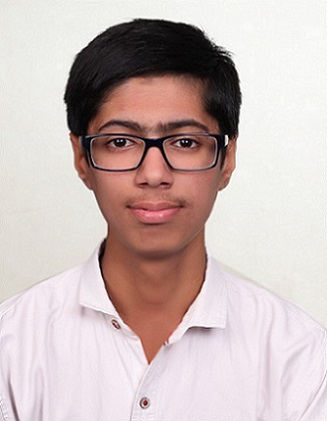
\includegraphics[width=0.5\linewidth]{52.png}
    \caption{Enter Caption}
    \label{fig:enter-label}
\end{figure}